%Classe du document, A4, police taille 12
\documentclass[a4paper,12pt]{article}

% Dictionnaire français, pour caractères spéciaux, tirets, caractères accentués
\usepackage[french]{babel}
\usepackage[utf8]{inputenc}
%Toujours plus d'accents
\usepackage[T1]{fontenc}
\usepackage{lmodern}
\usepackage{indentfirst}
%Pour créer des paragraphes random
\usepackage{lipsum}  
%bibliographie
%Le style dépend du projet, voir avec le grand chef
%A mettre à l'endroit où vous voulez la faire apparaitre
%Donc dans le code pas ici t'as vu
%\bibliographystyle{ieeetr}
%\bibligraphy{nom_du_fichier.bib}

%hauteur entre deux lignes
\baselineskip 200cm
%hauteur entre deux paragraphes
\parskip 2mm
%longueur d'indentation
\parindent 2mm
%(on utilise \indent et \noindent sinon)

%Gérer ses marges

%Facilement
\usepackage[margin=2cm]{geometry}

%Commentaire sur plusieurs lignes
\usepackage{verbatim}

%Précisément
%\usepackage[left=2cm , right=2cm, bottom=2cm, top=2cm, headheight=2cm]{geometry} 
%header c'est l'en-tête pas la marge supérieure

%Toujours plus précisément
%\addtolength{\oddsidemargin}{-0.5in}
%\addtolength{\evensidemargin}{-5cm}
%\addtolength{\topmargin}{-0.5in}

%Faires des articles  plusieures colonnes
\usepackage{multicol}
%Separation des colonnes
\setlength{\columnsep}{2cm}

%Avoir des entêtes et pieds de page stylés
\usepackage{fancyhdr}
\pagestyle{fancy}
%Pour enlever l'entête avec les sections
%\fancyhf{}

%Ca se fait sous format \<pos><type>{<contenu>}
%type c'est "head" ou "foot"
%pos pour position gauche "l", droite "r" ou centre "c"
%contenu c'est ce que tu mets dans dedans 
%marche aussi avec des images mais flemme
%mettre un trait
%\renewcommand{\footrulewidth}{1.5pt}

% Liens dans le document
\usepackage{hyperref}  
% Légendes dans les environnements "figure" et "float"
\usepackage{subcaption}
%La base pour faire des figures juste
\usepackage{graphicx}
\usepackage[export]{adjustbox}
\usepackage{wrapfig}
%Trucs utiles pour les maths
\usepackage{amsmath}

\begin{document}
\begin{titlepage}
    \begin{center}
        \vspace*{0.5cm}
        
\includegraphics[scale=0.1]{logo_ponts.jpg}\\
        \vspace{0.7cm}
        {\Large ÉCOLE NATIONALE DES PONTS ET CHAUSSÉES}\\
        \vspace{4cm}
        \rule\linewidth{0.05cm}
        {\huge Recherche Opérationelle\par}
        \rule\linewidth{0.05cm}
        \vspace{1cm}
        {\Large Projet \par}
        \vspace{0.8cm}
        %{\Large }\\
        \vspace{0.3cm}
        {\large \textit{Nicolas BESSIN}}\\
        \vspace{0.3cm}
        {\large \textit{Erwann ESTEVE}}\\
        \vspace{0.3cm}
        {\large \textit{Tidiane POLO}}\\
        \vspace{1.2cm}
        
    \end{center}
\end{titlepage}

\section{Questions}
%\begin {enumerate}
%\item { 
    \textit{Q1 }
    Les contraintes suivantes sur $\mu$ permettent la linéarisation de $\mu = \alpha \beta$ avec $\alpha \in \lbrace 0,1 \rbrace$ et $\beta \in \lbrack 0, M \rbrack$ : 
    \begin{equation*}
        \begin{cases}
            \begin{alignedat}{2}
                &\mu \in [0,M] && \quad \text{(domaine de définition)}  \\ 
                &\mu \leq \alpha M && \quad  \text{(impose } \mu = 0 \text{ si }  \alpha = 0 \text{)}\\
                &\beta - (1 - \alpha)M \leq \mu \leq \beta && \quad \text{(impose } \mu = \beta \text{ si }  \alpha = 1 \text{)}
            \end{alignedat}
        \end{cases}
    \end{equation*}
%}
%\item {
    \textit{Q2 }
    Les contraintes suivantes sur $\mu$ et $\alpha$ permettent la linéarisation de $\mu = [\beta]^{+}$ avec $\beta \in \lbrack -M, M \rbrack$ : 
    \begin{equation*}
        \begin{cases}
            \begin{alignedat}{2}
                &\mu \in [0,M], \alpha \in \lbrace 0,1 \rbrace && \quad \text{(domaine de définition)} \\ 
                &\beta \leq M \alpha \leq M + \beta && \quad \text{(impose } \alpha = 1 \text{ si }  \beta > 0, \alpha = 0 \text{ si } \beta < 0 \text{)} \\
                &\beta - (1-\alpha)M \leq \mu \leq \beta + (1-\alpha)M && \quad \text{(impose } \mu = \beta \text{ si }  \alpha = 1 \text{)} \\
                &\mu \leq \alpha M && \quad \text{(impose } \mu = 0 \text{ si }  \alpha = 0 \text{)}
            \end{alignedat}
        \end{cases}
    \end{equation*}
    Notons que $\alpha$ est indéterminé pour $\beta = 0$, mais qu'on a tout de même $\mu = 0= [\beta]^{+}$.
%}
%\item {

    \textit{Q3 }
    On introduit les variables binaires $y_\alpha$ et $y_\beta$, et la variable continue $y$.
    Le problème s'écrit alors :
    \begin{equation}
        \begin{alignedat}{2}
            \min _{\alpha, \beta, y_\alpha, y_\beta, y} & y \\
            \text{ s.c. } 
            &y \geq \alpha - 2M y_\alpha, & \quad& y \geq \beta - 2M y_\beta, \quad y_\alpha + y_\beta = 1 \\
        \end{alignedat}
    \end{equation}
    La contrainte $y_\alpha + y_\beta = 1$ assure  $y = \alpha$ ou $y = \beta$.
    De plus, puisque c'est un problème de minimisation, on a bien $y = min(\alpha, \beta)$. \\
    %\textit{N.B. : Nous avons trouvé cette élégante méthode à \underline{\href{https://doi.org/10.3390/math10020283}{ce lien}}.}
%}
%\item {
    \textit{Q4 }
    \begin{comment}
        On a le problème suivant : 
        \begin{equation}
            \begin{aligned}
                \min _{\alpha, \beta, \gamma} & \max (\alpha, \beta) + \gamma \\
                \text{ s.c. } & A(\alpha, \beta, \gamma)^T \leq b \\
            \end{aligned}
        \end{equation}
    \end{comment}
    On introduit la variable continue $\delta$ et les contraintes suivantes :$\qquad \delta \geq \alpha, \quad \delta \geq \beta $ \\
    Le problème initial s'écrit alors :
    \begin{equation}
        \begin{aligned}
            \min _{\alpha, \beta, \gamma, \delta}  \delta &+ \gamma \\
            \text{ s.c. }  A(\alpha, \beta, \gamma)^T \leq b, & \quad \alpha \leq \delta,  \quad \beta \leq \delta \\
        \end{aligned}
    \end{equation}
%}
%\item{
    \textit{Q5 }
    \underline{Remarque :} Pour la linearisation des termes en -min : $-min(a,b) = max(-a,-b)$ \\
    Pour linéariser les termes $p_f(v, x, y) c^c(C^f(v, x, y, z ,\omega))$, on doit distribuer la multiplication.\\
    \textit{N.B. : la justification de cette formulation du PLNE est trouvable étape par étape dans les commentaires du document linearSolverCode.jl} 
    \begin{align*}
        & \min_{x,y,z} cost^{cons}+ cost ^{ope} \\
         (x_{v,s}) \in \{0,1\}^{V^{s} \times S}, & (y_{e,q}^{land}) \in \{0,1\}^{E^0 \times Q}, (z_{e})\in \{0,1\}^{E^t}, (y_{e,q}^{sub}) \in \{0,1\}^{E^S\times Q}\\
        & \text{s.c. \text{ (1), (2), (3), (4)  (conditions du sujet)}} 
    \end{align*}
    \begin{equation}
        \begin{cases}
            \begin{alignedat}{2}
                & minusCapa_v \geq - \sum_{s \in S} r_s * x_{v,s}, \quad minusCapa_v \geq - \sum_{q \in Q_0} r_q * y_{e,q}^{land}  &&  \text{for } v \in V^s, e = (v_0, v)  \\
                & C_{v,\omega}^{n} \geq 0, \quad C_{v,\omega}^{n} \geq \pi_\omega * \sum_{t \in V^t} z_{v,t} + minusCapa_v  &&  \text{for } v \in V^s, \omega \in \Omega  \\
                & C^n_{\omega} = \sum_{v \in V^s} C_{v,\omega}^{nf} && \text{for } \omega \in \Omega \\
            \end{alignedat}
        \end{cases}
    \end{equation}
    \begin{equation}
        \begin{cases}
            \begin{alignedat}{2}
                & C_{v, \omega}^{ownFail} \in R^{V^s \times \Omega}_+ \\
                & C_{v, \omega}^{ownFail} \geq 0, \quad C_{v, \omega}^{ownFail} \geq \pi_\omega * \sum_{t \in V^t} z_{v,t} - \sum_{e = (v, \tilde{v}) \in E^S , q \in Q_0} r_q * y_{e,q}^{sub}  &&  \text{for } v \in V^s, \omega \in \Omega \\
            \end{alignedat}
        \end{cases}
    \end{equation}
    \begin{equation}
        \begin{cases}
            \begin{alignedat}{2}
                & (P_{u,v,\omega}^{sent}) \in R^{{V^s}^2 \times \Omega}, 1_{u,v,\omega}^{powerIsMin} \in \{0,1\}^{{V^{s}}^2 \times \Omega},  1_{u,v,\omega}^{cableIsMin} \in && \{0,1\}^{{V^{s}}^2 \times \Omega} \\
                & 1_{u,v,\omega}^{powerIsMin} + 1_{u,v,\omega}^{cableIsMin} = 1 && \text{for } (u,v) \in {V^s}^2, \omega \in \Omega \\
                & P_{u,v,\omega}^{sent} \geq \sum_{t \in V^t} z_{u,t} * \pi_\omega - 1_{u,v,\omega}^{cableIsMin} * P^{max} * N^{turbine} \\
                & P_{u, v, \omega}^{sent} \geq  \sum_{q \in Q^S} y_{e,q}^{sub} * r_q - 1_{u, v, \omega}^{powerIsMin} * P^{max} * N^{turbine} && e = (u, v) \\
            \end{alignedat}
        \end{cases}
    \end{equation}
    \begin{equation}
        \begin{cases}
            \begin{alignedat}{2}
                & C_{u, v, \omega}^{otherFail} \in R^{{V^s}^2 \times \Omega}_+ \\
                & C_{u, v, \omega}^{otherFail} \geq 0, \quad C_{u, v, \omega}^{otherFail} \geq \pi_\omega * \sum_{t \in V^t} z_{v,t} - P_{u, v, \omega}^{sent} + minusCapa_v
            \end{alignedat}
        \end{cases}
    \end{equation}
    \begin{equation}
        \begin{cases}
            \begin{alignedat}{2}
                & C^f(v, \omega) \in R^{V^s \times \Omega} && \\
                & C^f(v, \omega) = C_{v, \omega}^{ownFail} + \sum_{\substack{e = (v_0, \bar{v}), v \neq \bar{v}, \tilde{e} = (v, \bar{v})}} C_{v, \bar{v} \omega}^{otherFail} && \text{for } v \in V^s, \omega \in \Omega \\
            \end{alignedat}
        \end{cases}
    \end{equation}
    \begin{equation}
        \begin{cases}
            \begin{alignedat}{3}
                & (cost_{\omega}^{n}) \in R^{V_{s} \times \Omega} , (cost_{v,\omega}^{f}) \in R^{V^{s} \times \Omega} \\
                & cost^{cons} = \sum_{v \in V^s} \sum _{s \in S} c_s x_{vs} + \sum_{e \in E^0} \sum_{q \in Q_0} c_{eq} y_{eq}^{land} + \sum _{e \in E^S} \sum_{q \in Q_S} c_{eq} y_{eq}^{sub} + \sum_{e \in E^t} c_e z_e \\
                & cost_{\omega}^{n} \geq c^{0}C_{\omega}^{n} , cost_{\omega}^{n} \geq c^{0}C_{\omega}^{n} + c^{p}(C_{\omega}^{n}-C^{max}) \quad &&  \text{for } \omega \in\Omega, v \in V^{s} \\
                & cost_{v,\omega}^{f} \geq c^{0}Curt_{v,\omega}^{fail}, \quad cost_{v,\omega}^{f} \geq c^{0}C_{v,\omega}^{f} + c^{p}(C_{v,\omega}^{f} - C^{max}) \quad && \text{for } \omega \in\Omega, v \in V^{s} \\
            \end{alignedat}
        \end{cases}
    \end{equation}
    \begin{equation}
        \begin{cases}
            \begin{alignedat}{2}
                & (x_{v,s,\omega}^{timesCostF}) \in R^{V^{s} \times S \times \Omega},(y_{e,q, \omega}^{timesCostF}) \in R^{V^{s} \times Q \times \Omega} \\
                & cost^{max} = c^0  P^{max}  N^{turbine} + c^p  \lbrack P^{max} N^{turbine} - C^{max} \rbrack ^+ && \text{Pas une variable} \\
                & x_{v,s,\omega}^{timesCostF} \leq x_{v,s} * cost^{max}, \quad x_{v,s,\omega}^{timesCostF} \leq cost_{v, \omega}^{f} && \text{for } \omega \in\Omega, v \in V^{s}, s \in S\\
                & x_{v,s,\omega}^{timesCostF} \geq cost_{v, \omega}^{f} - (1 - x_{v,s})*cost^{max}, \quad x_{v,s,\omega}^{timesCostF} \geq 0 && \text{for } \omega \in\Omega, v \in V^{s}, s \in S\\
                & y_{e,q,\omega}^{timesCostF} \leq y_{v,q}^{land}*cost^{max}, \quad y_{e,q,\omega}^{timesCostF} \leq cost_{v, \omega}^{f} && \text{for } \omega \in\Omega, v \in V^{s}, q \in Q\\
                & y_{e,q,\omega}^{timesCostF} \geq cost_{v, \omega}^{f} - (1 - x_{v,s})*cost^{max}, \quad y_{e,q,\omega}^{timesCostF} \geq  0  \quad && \text{for } \omega \in\Omega, v \in V^{s}, q \in Q\\
            \end{alignedat}
        \end{cases}
    \end{equation}
    \begin{equation}
        \begin{cases}
            \begin{alignedat}{2}
                & (x_{v,s,\omega}^{timesCostNoF}) \in R^{V^{s} \times Q_{0}, \Omega}, (y_{e,q,\omega}^{timesCostNoF}) \in R^{V^{s} \times Q_{0}, \Omega} \\
                & x_{v,s,\omega}^{timesCostNoF} \leq x_{v,s}*cost^{max}, \quad x_{v,s,\omega}^{timesCostNoF} \leq cost_{\omega} ^n && \text{for } \omega \in\Omega, v \in V_{s}, s \in S\\
                & x_{v,s,\omega}^{timesCostNoF} \geq cost_{\omega} ^n - (1-x_{v,s})*cost^{max}, \quad x_{v,s,\omega}^{timesCostNoF} \geq 0 && \text{for } \omega \in\Omega, v \in V_{s}, s \in S\\
                & y_{e,q,\omega}^{timesCostNoF} \leq y_{v,q}^{land} * cost^{max}, \quad y_{e,q,\omega}^{timesCostNoF} \leq cost_{\omega} ^n \quad && \text{for } \omega \in \Omega, q \in Q_{0}, v \in V^{s} \\
                & y_{e,q,\omega}^{timesCostNoF} \geq cost_{\omega} ^n -(1-y_{v,q}^{land})*cost^{max}, \quad  y_{e,q,\omega}^{timesCostNoF} \geq 0 \quad && \text{for } \omega \in\Omega, q \in Q_{0}, v \in V^{s}\\
            \end{alignedat}
        \end{cases}
    \end{equation}
    \begin{equation}
        \begin{cases}
            \begin{alignedat}{2}
                cost^{ope} = & \sum_{\omega \in \Omega} \lbrack \sum_{v \in V^s} ( \sum_{s \in S} p_s x_{v,s,\omega}^{timesCostF} + \sum_{\substack{q \in Q^0, e = (v_0, v)}} p_q y_{e,q,\omega}^{timesCostF} ) \\
                &+ cost^n_{\omega} - \sum_{v \in V^s} ( \sum_{s \in S} p_s x_{v,s,\omega}^{timesCostNoF} + \sum_{\substack{q \in Q^{0}, e = (v_0, v)}} p_q y_{e,q,\omega}^{timesCostNoF} ) \rbrack \\ 
            \end{alignedat}
        \end{cases}
    \end{equation}

\textit{Q6}
On obtient pour small la solution optimale suivante, pour une valeur optimale de \textit{3246.97} :

\begin{figure}[h]
    \centering
    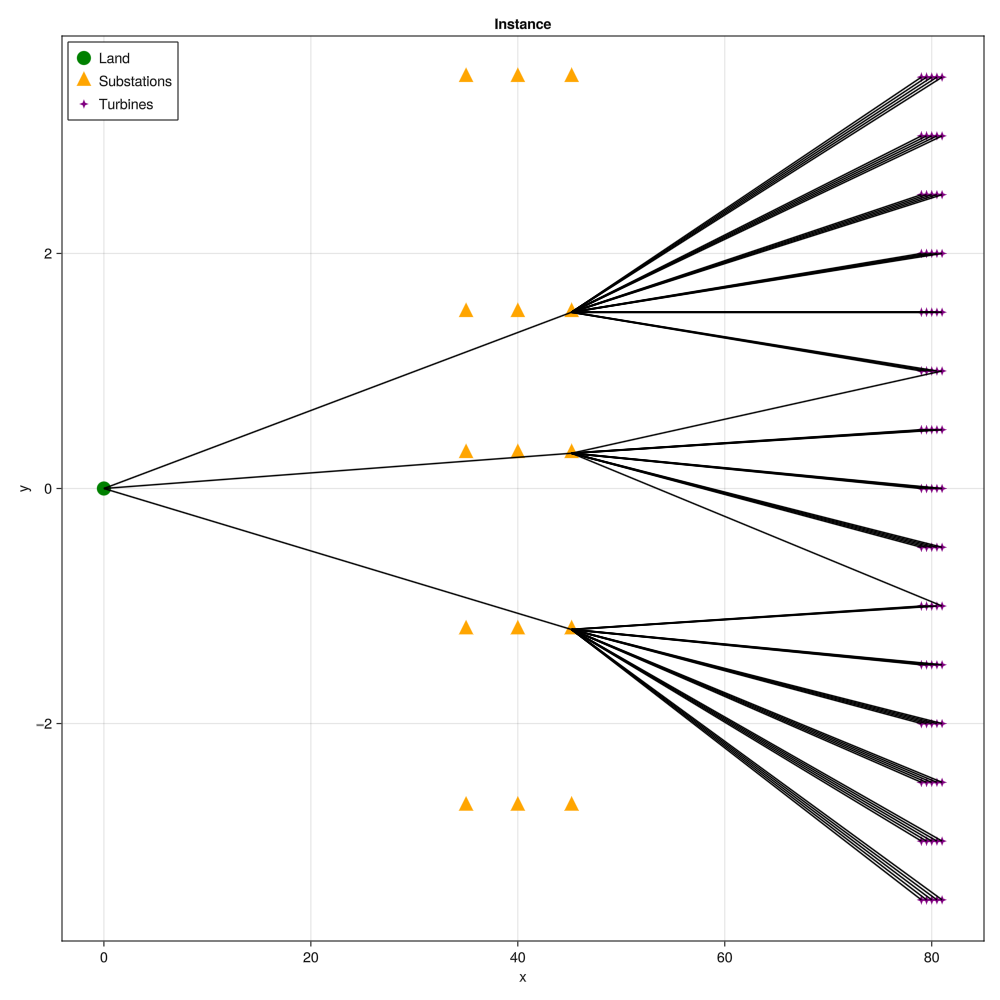
\includegraphics[scale=0.2]{small.png}
    \caption{Solution optimale pour l'instance small}
\end{figure}

\textit{Q7} Les \textit{indicator} rallongent le temps de calcul mais la solution optimale est la même. (cf document \textit{solverQuadraticIndicator.jl}, lignes 122 à 145). On peut en déduire que linéariser un problème est plus efficace, même si cela requiert un travail de linéarisation au préalable.

\textit{Q8}
On constate (cf \textit{Q6}) que les sites de sous-station utilisés sont les plus proches des éoliennes, et que les types de sous-station et de câbles utilisés sont les moins chers (voir figure 2).
De plus, plutôt que de regrouper toutes les éoliennes sur une même sous-station, la solution optimale les répartit sur trois sous-stations différentes, ce qui permet d'améliorer la résilience de la solution.
\section {Algorithm}
Une fois le solveur linéaire mis en place, le problème principal qui empêche de l'utiliser pour les instances medium, large et huge est la taille de celles-ci - en effet, le nombre de variables dans le modèle influe énormément sur le temps de calcul (et donc la possibilité de résoudre le problème). 
Ainsi nous avons implémenté la stratégie suivante :
\begin{itemize}
    \item Réduire la taille de l'instance avec différentes méthodes (voir ci-dessous).
    \item Résoudre le problème pour cette sous-instance avec le solveur linéaire
    \item Transformer la solution obtenue en une solution du problème initial. 
\end{itemize}
Les stratégies de réduction de taille que nous avons implémentées sont motivées par les observations suivantes que nous avons pu faire sur l'instance small :
seuls certains sites de sous-station sont utilisés (voir figure 1), seuls certains types de sous-station et de câbles sont utilisés (voir figure 2), et le nombre de scénarios est très grand (~100 pour small \& medium, ~1000 pour large \& huge).
\begin{figure}[h]
    \centering
    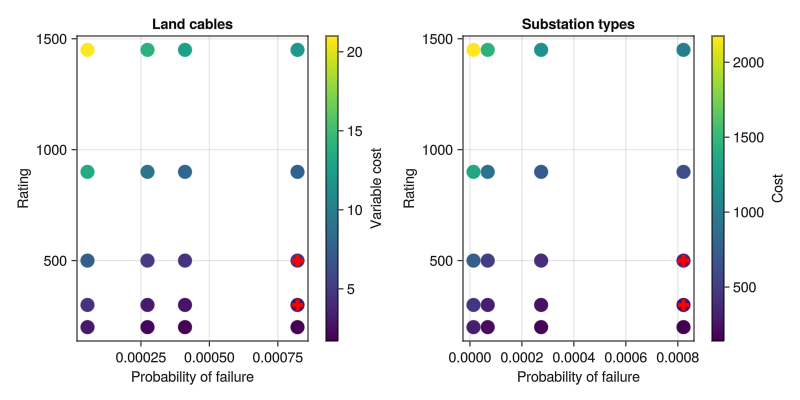
\includegraphics[scale=0.3]{small-types.png}
    \caption{Types des sous-stations et des câbles dans l'instance small - en rouge, les types effectivement utilisés dans la solution optimale}
\end{figure}
\begin{itemize}
    \item Ne garder que les sites de sous-station les plus proches des éoliennes (comme avec la solution optimale de l'instance small)
    \item Remplacer les multiples scénarios par un unique scénario (e.g. un scénario dont la puissance est $p = p_{min} + x(p_{max} - p_{min})$ avec $x$ un coefficient choisi. Avec $x = 1$, la solution est sur-dimensionée : les coûts de contruction sont trop élevés, et avec $x = 0$, la solution est sous-dimensionnée : les coûts d'opération sont trop élevés. On trouve une valeur "optimale" de $x$ à environ $ x = 0.99$.)
    \item Éliminer certains types possibles de sous-stations et / ou de câbles, en fonction de leurs probabilités de panne et de leurs coûts.
\end{itemize}

\begin{table}[h]
    \centering
    \begin{tabular}{|l|l|l|l|l|l|}
        \hline
        Nom & $ x_{vs} $      & $ y_{eq} $                         & $ z_{e} $        & \begin{tabular}[c]{@{}l@{}}Curtailing of $v $ \\ under $ \omega$ \end{tabular} \\ \hline
        Quantité & $|V^s| \times |S|$ & \begin{tabular}[c]{@{}l@{}} $ |Q^0| \times |V^s| $ \\ $ + |V^s|^2 \times |Q^s| $ \end{tabular} & $|V^s| \times |V^t| $ & $ |V^s| |\Omega| $ \\ \hline
        Nom      & $C^n(x, y, z, \omega)$ & \begin{tabular}[c]{@{}l@{}}Curtailing of $v $ \\ under $ \omega$  and failure of $v$ \end{tabular}  & Power sent from $v$ to $\tilde{v}$ & $C^f(v, x, y, z, \omega)$ \\ \hline
        Quantité & $ |\Omega| $ & $ |V^s| |\Omega| $                            & $ |V^s|^2 |\Omega| $            & $ |V^s| |\Omega| $              \\ \hline
    \end{tabular}
    \caption{Nombre de variables du problème / contraintes en fonction des tailles caractéristiques de l'instance}
\end{table}
\newpage
Le nombre de variables / contraintes - et donc le temps de résolution - du problème est donc en $O(|V^s| |S| + |V^s|^2 |Q^s| + |V^s| |Q^0| + |V^s| |V^t| + |V^s| ^ 2 |\Omega|)$. \\
L'intérêt de la stratégie de réduction de taille d'instance est donc d'obtenir des instances dont on peut trouver la solution optimale en un temps raisonnable, à l'aide du solveur linéaire.
Ces sous-instances étant extraites des instances initiales, la solution optimale de la sous-instance est une solution réalisable pour l'instance initiale, de coût supérieur à l'optimal.
(Mais relativement proches si la réduction de taille est bien faite.)

\begin{table}[h]
    \centering
    \begin{tabular}{l|l|l}
    Instance & \begin{tabular}[c]{@{}l@{}}small\\ $|V^s| = 15, |\Omega| = 100$\end{tabular} & \begin{tabular}[c]{@{}l@{}}small reduced\\ $|V^s| = 5, |\Omega| = 1$\end{tabular} \\ \hline
    Time (s) & 7654                                                                         & 1.4                                                                           \\ \hline
    Cost     & 3244                                                                         & 3244                                                                             
    \end{tabular}
    \caption{Temps de calcul \& résultat selon la réduction appliquée}
\end{table}


\begin{table}[h]
    \centering

    \begin{tabular}{l|llll}
    size & small (optimal)& medium       & large   & huge    \\ \hline
    cost & 3244          & 6472         & 8566    & 5583    \\
    gap  & $\leq 3.8 \%$ & $\leq 7.5\%$ & Unknown & Unknown \\ 
    \end{tabular}

    \caption{Meilleurs résultats obtenus pour les différentes instances.}

\end{table}

Le gap est calculé par rapport à la solution du relaché linéaire, et est donc une sur-estimation du gap par rapport à la solution optimale entière.
    (Pour large \& huge, nous n'avons pas pu calculer le gap, 16Go de RAM n'étant pas suffisant pour les résoudre.)

\textit{Le code source pour le projet est disponible sur \underline{\href{https://github.com/Nicolas-Bessin/ProjetREOP}{github}}.}

\end{document}